\documentclass[tikz,border=10pt]{standalone}
\usepackage{tikz}
\usetikzlibrary{positioning, arrows.meta}

\begin{document}
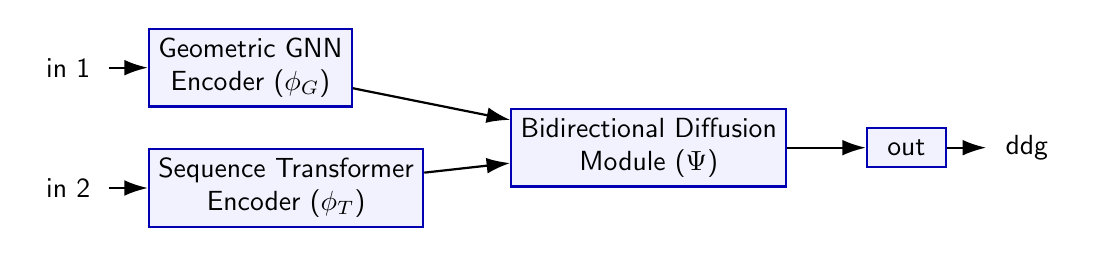
\begin{tikzpicture}[
    % --- Styles ---
    block/.style={
        rectangle,
        draw=blue!70!black,
        fill=blue!5,
        minimum width=1cm,
        minimum height=0.5cm,
        align=center,
        % font=\sffamily\bfseries,
        font=\sffamily,
        thick
    },
    block0/.style={
        rectangle,
        draw=white,
        fill=white,
        minimum width=1cm,
        minimum height=0.5cm,
        align=center,
        % font=\sffamily\bfseries,
        font=\sffamily,
        thick
    },
    arrow/.style={
        -{Latex[length=3mm, width=2mm]},
        thick
    }
]

% --- Nodes (relative positioning) ---
\node[block0] (input1) {in 1};
\node[block, right=0.5cm of input1] (cnn) {Geometric GNN \\ Encoder ($\phi_G$)};

\node[block0, below=1cm of input1] (input2) {in 2};
\node[block, right=0.5cm of input2] (gnn) {Sequence Transformer \\ Encoder ($\phi_T$)};

\node[block, below right=0.cm and 2cm of cnn.south east, anchor=north west] (diff)
    {Bidirectional Diffusion \\ Module ($\Psi$)};

\node[block, right=1cm of diff] (output) {out};
\node[block0, right=0.5cm of output] (out) {ddg};

% --- Arrows ---
\draw[arrow] (input1) -- (cnn);
\draw[arrow] (input2) -- (gnn);
\draw[arrow] (cnn) -- (diff);
\draw[arrow] (gnn) -- (diff);
\draw[arrow] (diff) -- (output);
\draw[arrow] (output) -- (out);

% --- Optional: feedback or vertical connection example ---
% \node[block, below=1.5cm of fusion] (aux) {Auxiliary Module};
% \draw[arrow, dashed] (fusion) -- (aux);
% \draw[arrow, dashed] (aux) |- (gnn);
% 
\end{tikzpicture}
\end{document}

